\documentclass[border=1pt,tikz,varwidth=\maxdimen]{standalone}

\usetikzlibrary{positioning,calc}

\usepackage{amsmath,mathtools}

\begin{document}
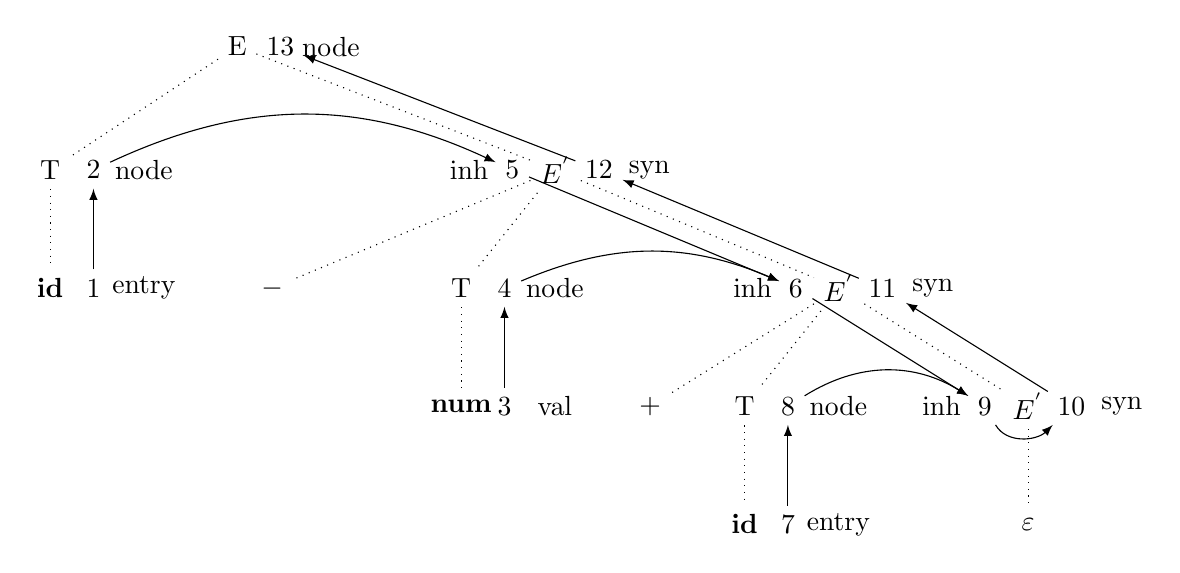
\begin{tikzpicture}[
  level/.style={sibling distance=2.4cm/#1},
  emph/.style={edge from parent/.style={dotted,draw}},
  norm/.style={edge from parent/.style={solid,draw}}
  ]
  \node (n01) {E};

  \node[below=1.2 of n01] (tmp) {};

  \node[left=2 of tmp] (n02) {T}
  child[emph] {
    node (n04) {\bf id}
  };

  \node[right=3.6 of tmp] (n03) {\(E^{'}\)}
  child[emph] {
    node (n05) {\(-\)}
  }
  child[emph] {
    node (n06) {T}
    child {
      node (n08) {\bf num}
    }
  }
  child[missing]
  child[emph] {
    node (n07) {\(E^{'}\)}
    child {
      node (n09) {\(+\)}
    }
    child {
      node (n10) {T}
      child {
        node (n12) {\bf id}
      }
    }
    child[missing]
    child[missing]
    child {
      node (n11) {\(E^{'}\)}
      child {
        node (n13) {\(\varepsilon\)}
      }
    }
  };
  \path[draw,dotted]
  (n01) -- (n02)
  (n01) -- (n03);

  \path (n04) ++(+0.55,0) node (s01) {1}  -- ++(+0.64,0) node {entry};
  \path (n02) ++(+0.55,0) node (s02) {2}  -- ++(+0.64,0) node {node};
  \path (n08) ++(+0.55,0) node (s03) {3}  -- ++(+0.64,0) node {val};
  \path (n06) ++(+0.55,0) node (s04) {4}  -- ++(+0.64,0) node {node};
  \path (n03) ++(-0.55,0) node (s05) {5}  -- ++(-0.55,0) node {inh};
  \path (n07) ++(-0.55,0) node (s06) {6}  -- ++(-0.55,0) node {inh};
  \path (n12) ++(+0.55,0) node (s07) {7}  -- ++(+0.64,0) node {entry};
  \path (n10) ++(+0.55,0) node (s08) {8}  -- ++(+0.64,0) node {node};
  \path (n11) ++(-0.55,0) node (s09) {9}  -- ++(-0.55,0) node {inh};
  \path (n11) ++(+0.55,0) node (s10) {10} -- ++(+0.64,0) node {syn};
  \path (n07) ++(+0.55,0) node (s11) {11} -- ++(+0.64,0) node {syn};
  \path (n03) ++(+0.55,0) node (s12) {12} -- ++(+0.64,0) node {syn};
  \path (n01) ++(+0.55,0) node (s13) {13} -- ++(+0.64,0) node {node};

  \path[-latex,black,draw]
  (s01) edge                 (s02)
  (s02) edge[out=25,in=155]  (s05)
  (s03) edge                 (s04)
  (s05) edge                 (s06)
  (s04) edge[out=23,in=157]  (s06)
  (s06) edge                 (s09)
  (s07) edge                 (s08)
  (s08) edge[out=32,in=148]  (s09)
  (s09) edge[out=300,in=225] (s10)
  (s10) edge                 (s11)
  (s11) edge                 (s12)
  (s12) edge                 (s13)
  ;
\end{tikzpicture}
\end{document}
